\section{RMHD Models of PWN}
\subsection{Simulating the plasma flow         (SK, OP, AL, BO, EA)}
\subsection{Radiative predictions, from particle transport models      (OP, AL, EA)}
\subsection{Gamma-ray binaries: pulsar winds interacting with a massive companion}
\subsubsection{Introduction}
The last decade revealed a new  a new group of gamma ray emitters, composed of a fast-rotating pulsar and a massive star. The emission, which peaks in the MeV band, arises from the shocked region between the stellar wind and the pulsar wind. Particle acceleration at the relativistic shock creates emission up to several TeV, the highest emission observed for binary systems. Fig.~\ref{fig:gamma_binary} presents a schematic view of interaction region. A handful of these systems have been discovered so far: PSR B1259-63 \citep{2005A&A...442....1A}, LS 5039 \citep{2005Sci...309..746A} ,LSI +61$^o$ 303 \citep{2006Sci...312.1771A}, HESS J0632+057\citep{2011ApJ...737L..11B}, 1FGL J1018.6-5856 \citep{2010ApJS..188..405A}, and more recently HESS J1832-093 \citep{2016MNRAS.457.1753E}. While pulsed emission has been observed for PSR B1259 (thanks to its wide orbit), and LSI+ 61$^o$ 303 has shown magnetar type flares \citet{ATEL}, the nature of the compact object is not firmly established in the other systems. However, given the very similar emission patterns, the colliding wind scenario is now firmly established. As such, the major aspects of the colliding wind structure and the high-energy emission mechanisms have been assessed, and while many questions remain, the study of  gamma-ray binaries has matured enough to become a new window on pulsar wind physics.  These systems provide a unique opportunity to study otherwise very elusive pulsar winds. The binary interaction typically takes place around a fraction of  AU from the pulsar (or about $10^4$ times the light cylinder), about 5 orders of magnitude closer than for pulsars interacting with the ISM.  Modeling strongly benefits from information provided by orbital variability and  the well constrained environment created by the companion star, both in terms of density and photons fields (at least compared to a typical region of the ISM).  While an excellent review can be found in \citet{2013A&ARv..21...64D}, this section provides some updates and focuses on how to determine the pulsar wind properties from the emission of gamma-ray binaries.


%\begin{figure}[h]  
%\centering
%  \includegraphics[trim=2cm 1cm 2cm .5cm, clip,width=.65\textwidth]{gamma_binary}
%\caption{Schematic view of a gamma-ray binary. The pulsar wind interacts with the stellar wind,  photon field and %circumstellar disk if the companion is a Be star.}
%\label{fig:gamma_binary}
%\end{figure}




\subsubsection {$\gamma$-ray binaries : puzzling observations}
While most of the energy is emitted in MeV photons (hence the name), gamma-ray binaries emit all the way from radio to a few TeV. Fig.~\ref{fig:SED_PSR} shows the high energy spectral energy distribution of PSR B1259-63 with emission resulting from the electrons accelerated at the shocks between the winds. Acceleration at the relativistic shock produces synchrotron emission (up to a few GeV) and Inverse Compton emission on seed photons of the massive star (up to a few TeV).   


In theses systems, most of the emission (with the exception of the low frequency radio band \citep{2015MNRAS.451...59M}) shows orbital variability. The right panel of  Fig.~\ref{fig:light_LS} shows lightcurves of LS 5039, a binary with a 3.9 day period:  X-ray and TeV emission show similar orbital variability, in opposition with the variability observed with $Fermi/LAT$.  The MeV emission in LS 5039, with an exponential cutoff at a few GeV before the harder but fainter TeV emission cannot be reconciled while assuming emission from a single population \citep{2008A&A...477..691D}. The different origin of the GeV and TeV emission is also suggested by the absence of emission below 200 GeV  in HESS J0632+057  \citep{2016arXiv160108216M} and around periastron in PSR B1259-63, while both show strong TeV emission.  

 LSI+61303 shows additional variability on superorbital timescales \citep{2012ApJ...747L..29C}, attributed to long-term variations in the Be disk surrounding the companion star \citep{2015A&A...575L...6P}. Interactions with the Be disk are likely responsible for the suborbital optical line variability in HESS J0632+057 \citep{2015ApJ...804L..32M}. 

In PSR B1259-63, which has a 3.4 year period, X-rays, TeV and radio flares are observed about 15 days before and after periastron. Optical spectroscopy indicates these flares are consistent with the disruption of the Be disk ask the pulsar crosses it \citep{2016MNRAS.455.3674V}.  About 60 days after periastron, $Fermi/LAT$ detects strong emission with no counterpart at any other wavelength \citep{2011ApJ...736L..11A}.  This flare, which contains almost all the spindown power of the pulsar,  has been confirmed at the 2014 periastron passage \citep{2015ApJ...811...68C} with a similar flux level and spectral shape but slightly different temporal evolution.  


Extended radio emission traces the contours of the shocked region \citep{2006smqw.confE..52D,2011ApJ...732L..10M}. Extended X-ray emission has also been found for most (if not all) of these systems but its origin remains unclear  \citep{2014AN....335..301K}. 


%\begin{figure}
%  \centering
%  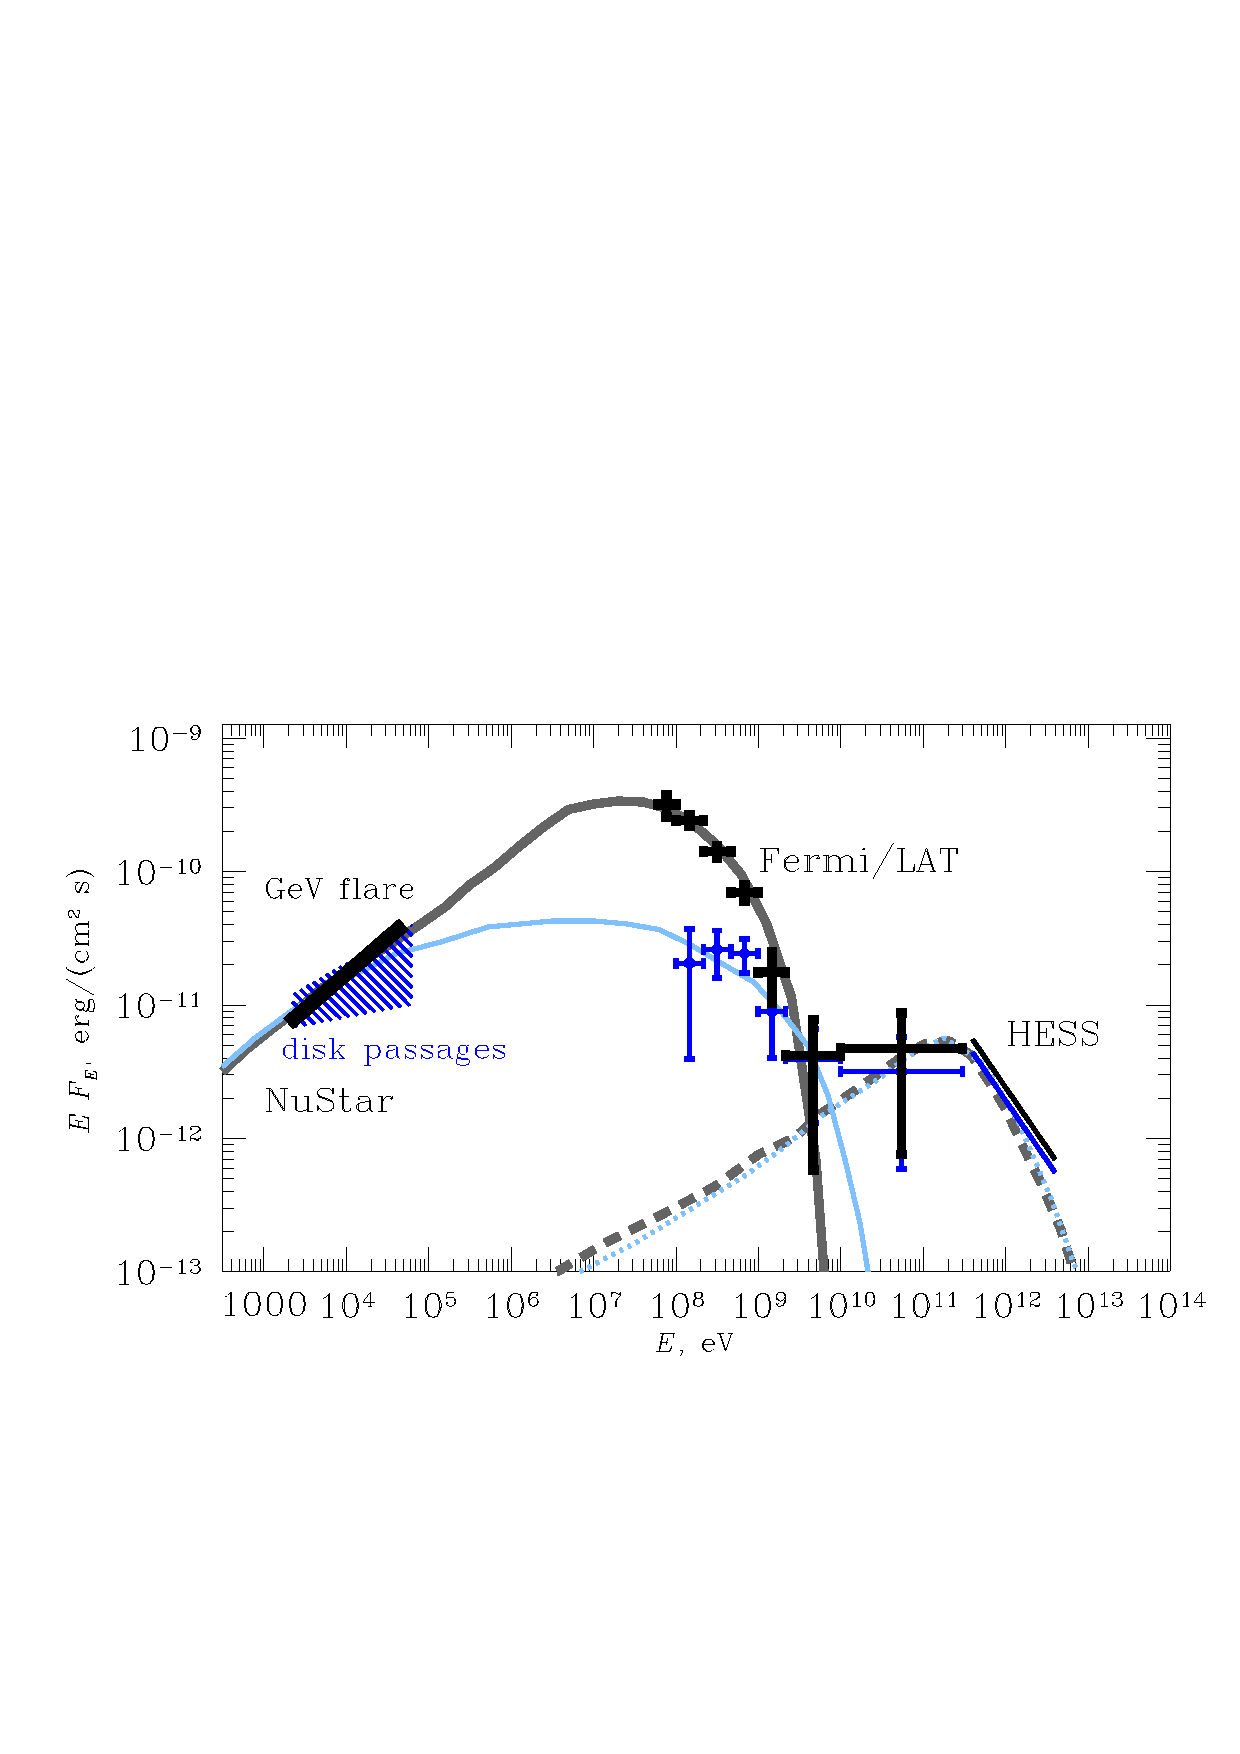
\includegraphics[width = .45\textwidth ]{PSRB_spectrum_broadband}
%\includegraphics[width=.4\textwidth]{ls5039_light}
%  \caption{Left : Spectral energy distribution of PSR B1259-63, during the disk passages (blue) and flares (grey) (from %\citet{2015MNRAS.454.1358C} ). Right : X-ray, GeV and TeV modulation for LS 5039. (Adapted from \citet{2009ApJ...697L...1K,2009ApJ...706L..56A} and \citet{2006A&A...460..743A} .)}
%  \label{fig:obs}
%\end{figure}


\section { Ingredients for successful models}


The wide variety of observational constraints is both a challenge an a tremendous opportunity to understand these systems.  Until recently, studies have either focussed on sophisticated one-zone emission models or aimed at reproducing the hydrodynamical  structure of the colliding wind region, with litte connexion to the non-thermal emission. While both approaches have had been fruitful, they have not been able to consistently reproduce the  orbital variability and spectral features from radio up to TeV.   The next sections describe both approaches and how they can be combined to yield a better understanding of pulsar wind physics.

The first ingredients are the non-thermal emission processes, dominated by leptonic processes \citep{2006A&A...456..801D}, causing a synchrotron bump and inverse Compton bump.  Models have included refined  representations of the ambient photon field, including self-Compton the on the nebula  \citep{2010A&A...519A..81C} and the infrared photons of the  Be disk when present  \citep{2012MNRAS.426.3135V}. Reproducing the TeV lightcurve of LS 5039 requieres anisotropic inverse Compton emission  \citep{2008A&A...477..691D} as an extended emission region. The latter is necessary to prevent complete absorption by pair production at  superior conjunction in LS 5039 (when the compact object is behind the massive stars).  Inverse-Compton pair cascades could extend the emission region \citep{2006MNRAS.371.1737B,2010A&A...519A..81C}. Or, the  emission could also result from one or more  distant emission regions \citep{2013A&A...551A..17Z}.  Similarly, the presence the absence of occultation features in the X-ray lightcurves suggests an extended emission region \citep{2007A&A...473..545B,2011MNRAS.411..193S}.  As the emission originates from the relativistic shocked pulsar wind, Doppler boosting is also at work at inferior conjunction (when the pulsar wind points toward the observer) and explains some of the GeV modulations \citep{2010A&A...516A..18D}. 


 Single zone models have so far failed to consistently reproduce the full variability of the systems, even when cascase emission is allowed. The exponential cutoff around a few GeV is hard to reconcile with the hard TeV emission. A single particle distribution with IC, synchrotron  and adiabatic  cooling fails to reproduce  this spectral feature \citep{2008MNRAS.383..467K,2013A&A...551A..17Z}.   The presence of an additional emission component has been suggested. While the GeV emission  is analogous to  pulsar magnetospheric emission observed by $Fermi$, it's orbital variations are hard to explain \citep{2012ApJ...749...54H}.   The emission of the unshocked pulsar wind \citep{2007MNRAS.380..320K}   has been considered but is insufficient \citep{2008APh....30..239S}.  A shocked mono-energetic  component have also been considered \citep{2013A&A...557A.127D}.  An alternate path is the presence of a different acceleration region, with different properties in terms of magnetic field, photon field and velocity structure \citep{2013A&A...551A..17Z}.

Over the years, it has become clearer that the only path towards fully understanding the emission in gamma-ray binaries would require an elaborate model for the geometry of the system, coupled with a refined model for the non-thermal emission. 

The flow dynamics in gamma-ray binaries are dominated by the double shock structure. It  shares many similarities with colliding stellar winds, which have been studied for decades. Simulations \citep{2009MNRAS.396.1743P,2011MNRAS.418.2618L} show strong instabilities which may  yield mixing in the winds \citep{2010MNRAS.403.1873Z}  and affect spiral structure expected at large scales \citep{2012A&A...546A..60L,2012A&A...544A..59B}.  

However, the relativistic nature of the pulsar wind affects the structure of the interaction region. Relativistic hydrodynamics yield more complex shock patterns, where parallel velocities (to the shock normal) play a role. Multidimensional simulations in the  ultrarelativistic regime of pulsar winds (Lorentz factor $\simeq 10^3-10^5$) are far beyond current computational and numerical capabilities. Some rescaling may be necessary even when focusing on the shocked winds,which have $\Gamma\lesssim 10$ close to the pulsar.  Simulations suggest a narrower opening angle for the pulsar wind \citep{2013A&A...560A..79L}, and a reacceleration of the pulsar wind up to its initial velocity \citep{2008MNRAS.387...63B}. Keeping in mind these intrinsic difficulties, relativistic simulations are crucial in order to determine Doppler boosting, which is a key ingredient to orbital modulation and maybe the GeV flares in PSR B1259 \citep{2012ApJ...753..127K}. Simulations suggest the presence of a back shock behind the pulsar, which can provide an additional site for particle acceleration, further away from the binary. They also indicate the presence of a large scale bubble as both winds interact with the ISM (add refs).





%\begin{figure}[h]
%  \centering
%  \includegraphics[width = .33\textwidth ]{emission_map}
%  \includegraphics[width = .63\textwidth ]{all_curves}
%  \caption{Left: TeV and X-ray emission maps for LS 5039 at superior and inferior conjunctions. Right: Simulations lightcurves for LS 5039 with a powerlaw particle distribution (black) and an additional mono-energetic component (grey). Images taken from \cite{2015A&A...581A..27D}.}
%  \label{fig:LS5039}
%\end{figure}

\citet{2015A&A...581A..27D} developed the first high energy emission model based on a fully three-dimensional relativistic simulations of LS 5039.  As explained in section \ref{sec:method}, the non-thermal emission is determined during post-processing, with a particle distribution injected at the relativistic shock and followed along the streamlines in the shocked pulsar wind. The model self-consistently represents adiabatic, inverse Compton and synchrotron cooling. The resulting emission takes into account pair creation, anisotropic Inverse Compton and directly benefits from the simulation to model Doopler boosting.  Fig. ~\ref{fig:LS5039} shows the resulting emission maps and lightcurves.  Comparison with observations suggested a strongly magnetized, rather slow pulsar wind ($\Gamma\simeq 10^3, \sigma \simeq 1$). While small discrepancies exist with observations, and radio emission won't be modeled properly without taking into account the magnetic field structure, the clear success of the combination of relativistic hydrodynamics with refined emission models shows the path forward in this field.



\subsection{Wisps as probes of the particle acceleration mechanism in the Crab nebula}
%*************************
%*************************
Pulsar Wind Nebulae (PWNe) are among the most powerful accelerators in the Galaxy, with the Crab producing particles up to PeV energies. 
It is a common opinion that the acceleration of those high energy particles might take place in the proximity of the wind termination shock (TS). However the termination shock is a very hostile environment for acceleration, due to its own nature of magnetized and relativistic shock. 
Relativistic shocks have indeed proven to be efficient accelerators only in two cases: when the shock is quasi parallel, in particular when it is sub-luminal (meaning that the angle between $\vec{B}$ and $\vec{v}_\mathrm{shock}$ is $\theta\ll\theta_c\simeq 1/\gamma_\mathrm{shock}$), or when the shock is poorly magnetized, with the magnetization $\sigma$, defined as the ratio of Poynting flux to particle kinetic energy flux in the wind, below $\sim 10^{-3}$.

The observed spectrum of the Crab nebula, similar to other PWNe, seems to suggest different acceleration mechanisms for low and high energy emitting particles, since it is a broken power law $N(E)\propto E^{-\gamma_e}$, with $\gamma_e\sim 1.5$ at low energies (below $\sim 0.5$ eV) and $\gamma_e\sim 2.2$ at higher ones (up to a few GeV).

At present, two main candidates have been invoked as possible mechanisms for particle acceleration at the Crab TS.
%------ Driven MagREC --------------------

The slope of the radio component is compatible with driven magnetic reconnection. 
This mechanism was largely investigated by \citet{Sironi:2011} and \citet{Sironi:2013}, who have performed numerical simulations compatible with the Crab nebula's shock conditions. 

They assume that the striped morphology of the pulsar wind is maintained all the way to the TS, where the compression leads the magnetic field to reconnect. 
Reconnection islands form in the flow and particles can be accelerated by the un-screened electric field. 
The properties of the resulting spectrum depend on the flow magnetization and on the ratio between the wavelengths of the stripes and the particle Larmor radii. 
This ratio can be connected to the value of the pulsar pair multiplicity $\kappa$, and the result in the case of the Crab nebula is that, in order to reproduce the observed radio spectrum, a magnetization of $\sigma\gtrsim 30$ and a multiplicity of $\kappa \gtrsim 10^8$ are needed. The pulsar pair multiplicity $\kappa$ represents the rate at which particles are generated in the pulsar magnetosphere, namely it is defined as the number of pairs produced by a single primary electron that emerges from a polar cap of the pulsar. 

The main problem with this scenario is that it is very difficult to explain such a high value of the multiplicity: from observations and theoretical models we expect much smaller values, with $\kappa\sim 10^6$ at most. 
The only possibility to reduce the expected value of $\kappa$ is to accelerate particles near the polar cusps of the TS, where the shock front is nearer to the pulsar, and as a consequence the particle density is much higher (it decreases as $\approx 1/r^2$). 
On the other hand, no stripes are expected to be present at these locations, and reconnection can only be obtained thanks to O-point dissipation.

Moreover, a wind with the required high number of pairs, $\kappa\sim10^8$, is expected to reconnect well before the TS, causing the magnetization to lower well below the required minimum for the mechanism to be viable \citep{Amato:2014}. 

%------    DSA (Fermi I like acceleration)     --------------------

A different mechanism can be invoked to account for the much steeper high energy component of the spectrum. A photon index of $\gamma_e \simeq 2.2$ is in fact what one expects from Diffusive Shock Acceleration (DSA), i.e. Fermi I like acceleration at relativistic shocks. 
Contrary to driven magnetic reconnection, DSA is effective only if the magnetization is sufficiently low, in particular $\sigma \lesssim 10^{-3}$ is required \citep{Sironi:2009}. 
MHD simulations taught us that, if the emission from Crab has to be reproduced, this condition can only be realized in a thin latitude strip around the pulsar equator or in the vicinities of the polar axis, while at intermediate latitudes the flow magnetization must be substantially larger than this, likely $\sigma$ of order a few \citep{Komissarov:2013}. 
Therefore, at least DSA can only be effective in a few sectors of the shock, where magnetic dissipation is sufficiently strong so as to ensure a local condition of quasi-unmagnetized plasma \citep{Amato:2014}.

%----- OTHER POSSIBILITIES -------------------------------------
The other possibility that has received some attention in the literature is resonant absorption of ion-cyclotron waves in a ion-doped plasma. This requires that most of the energy of the wind is carried by ions and its viability does not depend on the value of the magnetization. 
The idea is that pairs were accelerated by resonant absorption of the cyclotron radiation emitted by ions in the wind, which are set into gyration by the enhanced magnetic field at the shock crossing \citep{Amato:2014}.

However, since at present there are no strong indications of a leading role of ions in the pulsar wind energetics, or that ions are present at all, this possibility would not be addressed in the present discussion.

%++++++++++++++++++++++++++++++++
\subsubsection{Wisps from Crab}
%++++++++++++++++++++++++++++++++

The inner region of the Crab nebula has been known to be highly variable at optical wavelengths since the late 60s, when \citet{Scargle:1969} first identified some bright, arc-shaped and variable features, that he named \enquote{wisps}. 
They appear to be periodically produced at about the expected location of the TS, which can be seen as the first bright ring surrounding the central dark region of the pulsar wind, and then move outwards with mildly relativistic velocities, as one expects for a post-shock hydrodynamic flow. 
Their typical period between appearance close to the TS and disappearance in the bulk of the nebula can be of the order of days, months or even years, depending on the energy band in which they are observed (X-rays, optical or radio respectively).
They also appear to be more prominent in the north-west sector than in the south-east.

Few years after the first wisps identification, the properties of such features were extensively studied at different wavelengths, in particular focusing on radio and optical bands, and more recently also on the X-ray band. 
The most important conclusion was that wisps at different wavelengths are not coincident and that they are seen to propagate at various speeds \citep{Bietenholz:2004,Schweizer:2013}.
The observed discrepancies between radio and optical wisps led \citet{Bietenholz:2004} to conclude that the two populations must have a different acceleration mechanism and/or site, and possibly the same conclusion might be drawn for X-ray wisps.


\subsubsection{Wisps as probes of the particle acceleration}

As we discussed previously, the different acceleration mechanisms proposed require very different physical conditions to be viable, which are not realized everywhere along the shock surface. Identifying the location at which particles are accelerated can then put strong constraints on the acceleration mechanism at work.

One way to test different scenarios of acceleration is by comparison with observations of the variability they entail in the inner nebula at various frequencies: since wisps are seen to start so close to the TS, at least at optical and X-ray frequencies, where radiative losses are important, they trace freshly injected particles, and in the simulated maps, their appearance and motion depends on the location at which the emitting particles are injected in the nebula.

In \citet{Olmi:2014} it was shown that wisp properties at radio wavelengths are well reproduced without invoking \emph{ad hoc} mechanisms, with the bulk flow of the nebula acting as the main driver for the observed wisps appearance and motions. 
In MHD models, wisps appearance is thus totally due to the combined effects of the locally enhanced magnetic field, just downstream of the TS, and the Doppler boosting effect, since channels with significant $v/c$ form along oblique sectors of the shock surface.
In particular, Doppler boosting is responsible for the angular profile of wisps, as well as for the enhanced brightness of the front side of the nebula with respect to the back side, that appears to be very faint. 
The intensity contrast between distinct wisps is, on the contrary, strongly connected to the local magnetic field strength.

Within an MHD description, the fact that wisps arise at different wavelengths with different properties (different locations and outward velocities) suggests a difference in the acceleration sites of the particles responsible of such emission.
In fact, assuming that the emitting particles are all accelerated at the TS, including the radio component, the discrepancies can only be explained by choosing different acceleration regions along the TS for distinct distributions. 
If particles with different energies are injected at different latitudes along the TS, the paths induced by the post-shock flow structures, and the adiabatic and synchrotron losses, will also be different, and features at different energies are expected to be not coincident, as observed.

In \citet{Olmi:2015} axisymmetric relativistic  MHD simulations are used to constrain the acceleration sites of particles responsible for the observed wisps at the different frequencies in the Crab nebula. 

Considering several different scenarios, with particles of different energies being injected in different sectors of the TS, with polar and equatorial cones defined with various angular extents, wisp properties are extracted on top of the simulated emission maps at various wavelengths.

The entire Crab nebula is simulated up to its present age ($\sim 1000$ yr), with outputs sampled with monthly frequency during the last 10 years of evolution. 
In analogy with \citet{Schweizer:2013}, wisp intensity profiles are extracted from radio, optical and X-ray emission maps from a $3\arcsec$ wide slice centered on the polar axis in the upper hemisphere of the nebula, where wisps are seen to be more prominent.
For ease of comparison with observational data, profiles are also convolved with the appropriate instrumental PSF (relative to the instrument used for the data considered for comparison in each band) and only intensity peaks with $I\geq I_\mathrm{max}/3$ are taken into account, where $I_\mathrm{max}$ is the maximum value of the intensity in each map. 
This cut off is applied in order to remove the background of weaker variations, that are not useful for the comparison with data. 

This procedure is then repeated for each output in the 10 years of the considered interval, and for each one of the defined cases for particles injection, namely:
\begin{enumerate}[(1)]
	\item  $\;$ particles are injected uniformly along the entire shock front, for all the three families;
	\item  $\;$ particles are injected in a wide equatorial sector along the shock ($\theta \in \left[ 20^o, 160^o \right]$) or in the opposite narrow polar one ($\theta \in \left[ 0^o, 20^o \right]\cup\left[ 160^o, 180^o \right]$);
	\item  $\;$ particles are injected in a narrow equatorial sector ($\theta \in \left[ 70^o, 110^o \right]$) or in the opposite wide polar one ($\theta \in \left[ 0^o, 70^o \right]\cup\left[ 110^o, 180^o \right]$).
\end{enumerate}

The polar and equatorial angular sectors of case (2) and case (3) are represented, respectively, by the green and red cones of Fig.~\ref{fig:ts}, where the structure of the velocity field is shown in the proximity of the TS.

%\begin{figure}
%\centering
% 	\includegraphics[scale=0.55]{ts.eps}
%\caption{Plot of the flow structure, with colors indicating the velocity magnitude in terms of $c$ and arrows the velocity field direction. The TS front is highlighted by the blue contour line of $0.99c$. Sectors corresponding to case (2) (polar) and case (3) (equatorial) are represented, respectively, by the green and red cones.} 
%\label{fig:ts}
%\end{figure}

Reasons for these prescriptions for the injection sectors are in order. Equatorial sector of case (3) roughly represents the wind striped region in the considered wind model (for a complete description see \citet{Olmi:2014}), while polar sector of case (2) mimics a scenario in which particles can be accelerated in the low-$\sigma$ region around the polar axis thanks to Fermi I acceleration or O-point dissipation.

\subsubsection{Wisp profiles in the different scenarios}

The three hypotheses are tested for radio, optical and X-ray particle families.
In particular two different distribution functions are defined to account for radio and X-ray emission, while the optical one is obtained as a mixed contribution of the other two. 
Since radio and X-ray distribution functions are normalized in order to fit the complete integrated spectrum of Crab, the optical spectrum is naturally determined as the superposition of radio and X-ray contributions.

Radio particles are injected with the following spectrum:
\begin{equation}
f_{0\mathrm{R}}(\epsilon_0)\propto \left\{
\begin{array}{lcl}
0 & {\rm if} & \epsilon_0 < \epsilon_{\rm minR}, \\
\epsilon_0^{-p_\mathrm{R}} \exp(-\epsilon_0/\epsilon_\mathrm{R}^*) &  {\rm if} & \epsilon_0 > \epsilon_{\rm minR},\\
\end{array}
\right.
\end{equation}
and X-ray ones with:
\begin{equation}
 f_{0\mathrm{X}}(\epsilon_0)\propto \left\{ 
 \begin{array}{lcl}
 0 & {\rm if} & \epsilon_0 < \epsilon_{\rm minX}, \\
\epsilon_0^{-p_\mathrm{X}} \exp(-\epsilon_0/\epsilon_\mathrm{X}^*) &  {\rm if} & \epsilon_0 > \epsilon_{\rm minX}, \\
\end{array}
\right.
 \label{eq:Xpart}
\end{equation}
 where $\epsilon_0$ is the Lorentz factor of the particle at the injection site.
 
Power-law indices and cut-off energies that appear in the previous formulas, are all determined based on the comparison of the simulated emission with data. The best set of those parameters resulted to be: $p_\mathrm{R}=1.6$, $\epsilon_{\rm minR}=10^3$, $\epsilon_\mathrm{R}^*=2 \times10^6$, $p_\mathrm{X}=2.8$, $\epsilon_{\rm minX}=1.5 \times 10^6$ and $\epsilon_\mathrm{X}^*=10^{10}$.


%\begin{figure}
%\centering
% 	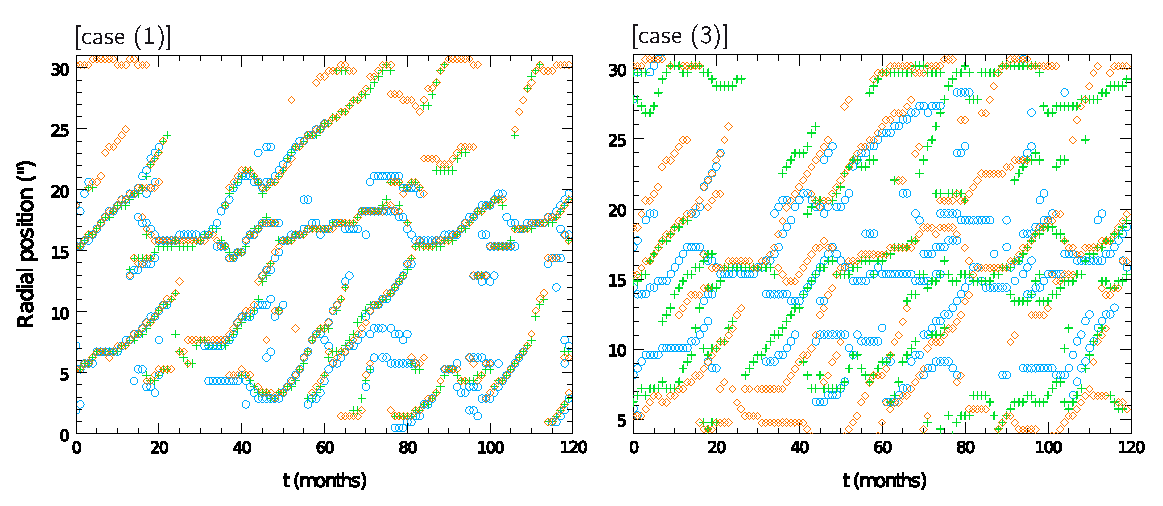
\includegraphics[scale=0.62]{case13-mod.eps}
%\caption{Radial positions of the local intensity maxima (in arcseconds) as a function of time (in months) with orange diamonds identifying radio wisps ($\nu_r=5$ GHz), green crosses optical ones ($\nu_o=3.75 \times 10^{14}$ Hz) and light-blue circles for X-rays (1 keV). 
%On the left case (1) is shown. On the right case (3) is shown, with X-ray particles injected in the equatorial zone and radio ones injected in the complementary sector.} 
%\label{fig:wisp1}
%\end{figure}

The first interesting point to look at is the difference between wisps profile under case (1) (i.e. uniform injection at TS) and one of the other two cases. In Fig.~\ref{fig:wisp1} wisp profiles are shown as plots of the radial position of the intensity maxima as a function of time, with case (1) on the left and case (3) (X-ray particles injected in the equatorial sector and radio in the polar one) on the right.
As expected, wisps appear to be coincident at the different wavelengths in the hypothesis of case (1). 
This is no more true as soon as particles of different families are injected in different sectors of the shock, as can be easily see in the plot on the right.

%\begin{figure}
%\centering
% 	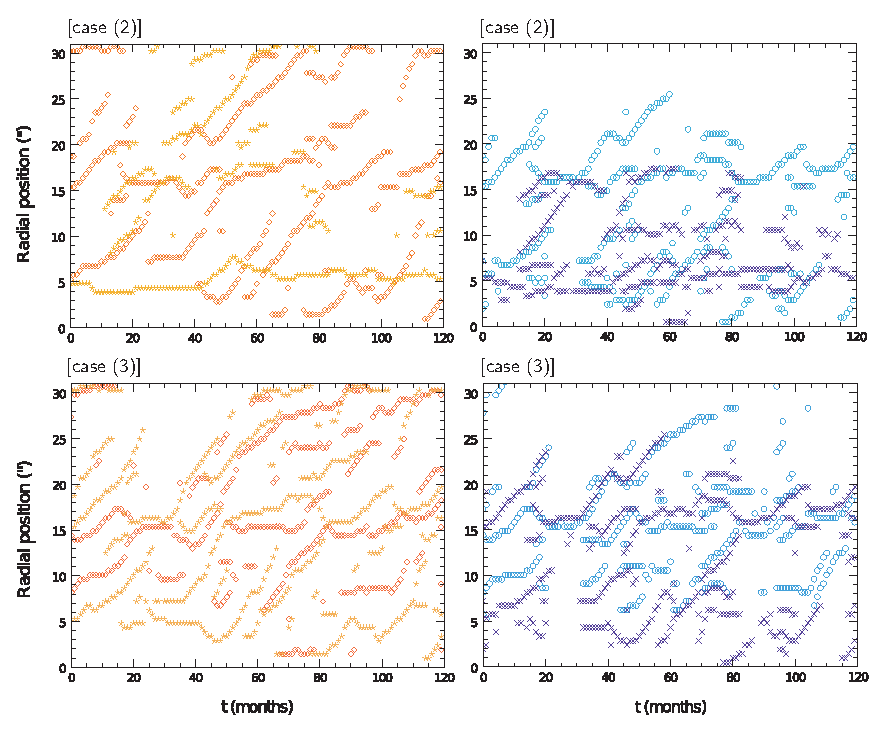
\includegraphics[scale=0.825]{cfr-cases.eps}
%\caption{Radial position of the local intensity maxima as a function of time for case case (2), in the upper row, and case (3), in the bottom one. On the left, different possibilities for the injection of radio particles are shown. Stars and diamonds represent, respectively, polar and equatorial injection. On the left-hand side, the same cases are shown for X-ray particles: violet crosses are used for polar injection and light blue circles for equatorial one.} 
%\label{fig:wisp2}
%\end{figure}

Excluding the case of uniform injection, which clearly does not reproduce the expected behavior of wisps, the remaining  possibilities are case (2) and (3). 
All the different scenarios of these two cases are shown and compared in Fig.~\ref{fig:wisp2}. 
Here particles responsible for radio and X-ray wisps are injected either in the polar sector (stars and crosses) or in the equatorial region (diamonds and circles).

When particles are injected in the wide equatorial region of case (2), wisps appear to be almost identical of those of the uniform injection case. 
On the contrary, particles injected in the narrow polar sector are not seen to produce wisp-like features, with the most prominent one being a quasi-stationary structure at a distance of $5\arcsec$ from the pulsar, which is something very different from what observations show.

Under hypotheses of case (2) is thus impossible to define two non coincident sectors in which radio and X-ray particles can be injected, so as to give rise to different wisps at the different energies.

Finally, in the bottom row of the same Fig.~\ref{fig:wisp2}, the alternative injection scenarios considered in case (3) are shown. 
Here wisps appear in any case, no matter whether particles are injected in the wide polar sector or they are injected in the narrow equatorial region. 
The strongest constraint for discriminating between the possibilities comes from \citet{Schweizer:2013}, 
where X-ray wisps were shown to be present only beyond $\sim 6\arcsec$ from the pulsar. 
The only case in which this behavior is correctly reproduced is when X-ray particles are injected in the equatorial region, which approximatively corresponds to the striped zone of the wind, where dissipation of magnetic field is most efficient.
This may indicate that X-ray particles are produced via Fermi I acceleration in the striped zone, where magnetization can be low enough to make this mechanism viable.

Outward apparent velocities of wisps at the different frequencies have also been investigated for case (3), leading to a range of $0.08c \lesssim v \lesssim 0.38c$, which is in good agreement with the one predicted by observations.

Strong constraints on radio emission are on the other hand very difficult to draw, and the only case that can be effectively excluded is the one in which radio particles are injected in a narrow polar cone. 
But, in order to have non coincident wisps at the different wavelengths, radio particles must be accelerated elsewhere than the equatorial region of case (3). 
The remaining possibilities are thus that acceleration happens in a wider equatorial region or in the complementary polar zone with respect to X-ray particles, where conditions for driven magnetic reconnection to be active might be locally satisfied.
%**************************
%**************************
